\documentclass[11pt,a4paper]{article}

\usepackage[T1]{fontenc}
\usepackage[utf8]{inputenc}
\usepackage[margin=2.4cm]{geometry}
\usepackage{graphicx}
\usepackage{booktabs}
\usepackage{amsmath,amssymb}
\usepackage{xcolor}
\usepackage{tcolorbox}
\usepackage{caption}
\usepackage{float}
\usepackage{enumitem}
\usepackage{array}
\usepackage[hidelinks]{hyperref}

\definecolor{kuetblue}{RGB}{20,60,110}
\definecolor{softgrey}{RGB}{245,245,247}

\captionsetup{font=small,labelfont=bf}
\setlist{itemsep=2pt,parsep=0pt,topsep=3pt}

\newtcolorbox{keybox}[1]{colback=softgrey,colframe=kuetblue,fonttitle=\bfseries,
  title={#1},boxrule=0.6pt,left=6pt,right=6pt,top=4pt,bottom=4pt}

\begin{document}

%========================================================= TITLE PAGE
\begin{titlepage}
\centering
\vspace*{1.0cm}

{\Large\bfseries Khulna University of Engineering \& Technology}\\[3pt]
{\large Department of Computer Science and Engineering}\\[1.5cm]

\rule{\textwidth}{1pt}\\[10pt]
{\LARGE\bfseries A Machine Learning Approach to\\[6pt]
Scoring and Ranking University Websites}\\[10pt]
{\large A Seven-Dimension Scoring Model and a Comparative Study\\of Twelve Regression Algorithms}\\[8pt]
\rule{\textwidth}{1pt}\\[1.3cm]

{\large\bfseries Course:} Machine Learning Laboratory\\[2pt]
{\large\bfseries Course Code:} CSE 4112\\[1.4cm]

{\large\bfseries Submitted By}\\[8pt]
\begin{tabular}{ll}
\toprule
\textbf{Name} & \textbf{Roll} \\
\midrule
Faisal Ahmed          & 2107061 \\
Al Shariar Hossain    & 2107066 \\
Md. Rubayet Nabil     & 2107073 \\
Khadimul Islam Mahi   & 2107076 \\
Abhijeet Deb Nath     & 2107083 \\
Afifa Sultana Offa    & 2107087 \\
\bottomrule
\end{tabular}\\[1.3cm]

{\large\bfseries Submitted To}\\[6pt]
\fbox{\parbox{0.55\textwidth}{\centering\vspace{3pt}
\textcolor{red}{\textbf{[ SUPERVISOR NAME AND DESIGNATION ]}}\\[2pt]
\small Department of Computer Science and Engineering\\
Khulna University of Engineering \& Technology\vspace{3pt}}}\\[1.2cm]

\vfill
{\large Date of Submission: \today}
\end{titlepage}

%========================================================= ABSTRACT
\section*{Abstract}

University websites are the primary interface between an institution and a prospective
student, yet their quality is rarely measured systematically. This project develops an
automated method for scoring and ranking them.

We collected 1,230 university landing pages worldwide, each described by 69 measurable
attributes, and reduced them to a clean modelling dataset of \textbf{1,225 universities and
71 features}. We then defined a \textbf{seven-dimension scoring model} that converts those
attributes into a website quality score from 0 to 100. The dimensions are organised around
what a prospective student needs from the site --- what can be studied, how to apply, whether
the institution is active, whether the site can be navigated, used, trusted and read --- and
are combined as a weighted sum subject to two gating rules. Four attributes are mapped
through explicit non-linear response curves, because their relationship with quality is not
monotone.

The dataset was split \textbf{80\% training / 20\% testing}, stratified on score band, and
\textbf{twelve regression algorithms} were trained and compared under identical conditions.
Performance ranged from $R^2 = 0.786$ (k-nearest neighbours) to $R^2 = 0.992$ (LightGBM).
After grid-search tuning, the selected LightGBM model achieves $R^2 = 0.993$, MAE $= 1.11$
score points and Spearman $\rho = 0.993$ on the 246 held-out universities.

The comparative study yields a finding of practical interest. The separation between
algorithm families is not random: it is concentrated entirely on the universities to which a
gating rule applies. On those 36 test cases, linear regression is wrong by 6.41 points on
average against 1.07 for LightGBM --- a $6\times$ difference --- because a weighted sum
cannot express a hard cap while a decision tree can. Gain-based importance analysis confirms
that the tuned model independently recovered the gate: the single navigation attribute that
triggers it accounts for 26\% of all loss reduction.

\vspace{4pt}
\noindent\textbf{Keywords:} website quality assessment, regression, model comparison,
feature engineering, gradient boosting, university ranking.

\tableofcontents
\newpage

%========================================================= 1
\section{Introduction}

\subsection{Motivation}

For a prospective student, a university's website is often the only source of information
available before applying. It determines whether they can find the programmes on offer, learn
the admission requirements, discover a deadline, or contact a human being. A poorly organised
site is not a cosmetic problem; it is a barrier to access.

Despite this, website quality is usually assessed by manual inspection --- slow, subjective
and impossible to apply at scale. This project asks whether the assessment can be automated:
whether a set of attributes that a program can extract from a landing page is sufficient to
predict a meaningful quality score.

\subsection{Problem statement}

\begin{center}
\begin{tabular}{c@{\hspace{7pt}}c@{\hspace{7pt}}c@{\hspace{7pt}}c@{\hspace{7pt}}c}
\fbox{\parbox{3.1cm}{\centering\small\textbf{INPUT}\\[2pt]71 measured\\attributes of one\\university landing page}}
& $\longrightarrow$ &
\fbox{\parbox{2.9cm}{\centering\small\textbf{MODEL}\\[2pt]trained\\regressor}}
& $\longrightarrow$ &
\fbox{\parbox{3.7cm}{\centering\small\textbf{OUTPUT}\\[2pt]website score $0$--$100$\\grade A+ \dots F\\global / regional / country rank}}
\end{tabular}
\end{center}

\noindent This is a \textbf{supervised regression} problem. Given the attribute vector of a
landing page, predict its website quality score. Because the deliverable is a league table,
rank-order agreement (Spearman $\rho$) is treated as the primary metric alongside $R^2$ and
mean absolute error.

\subsection{Objectives}

\begin{enumerate}
\item Collect and clean a global dataset of university landing-page attributes.
\item Define a transparent, reproducible scoring model that converts attributes into a
      0--100 website quality score reflecting a prospective student's needs.
\item Split the data 80/20 and train a broad range of regression algorithms on identical
      inputs.
\item Compare their performance and, more importantly, \emph{explain} why they differ.
\item Produce global, regional and country rankings, and analyse what drives a website's score.
\end{enumerate}

\subsection{Contributions}

\begin{enumerate}
\item A seven-dimension scoring model with documented weights, two gating rules and four
      non-linear response curves (Section~\ref{sec:scoring}).
\item A controlled comparison of twelve regression algorithms across six model families on
      the same 80/20 split (Section~\ref{sec:comparison}).
\item An error analysis that attributes the performance gap between families to a specific,
      demonstrable mechanism rather than to model capacity in the abstract
      (Section~\ref{sec:why}).
\item A ranking of 1,225 university websites with an interpretable account of what drives the
      score (Sections~\ref{sec:importance}--\ref{sec:rankings}).
\end{enumerate}

%========================================================= 2
\section{Dataset and Preparation}

\subsection{Source data}

The raw dataset consists of 1,230 university landing pages, each described by 69 attributes
extracted automatically, organised into eleven groups: header and navigation, rankings and
recognition, notices and updates, events and media, page content, footer, visual design,
service interaction, technical performance, SEO metadata and accessibility. Attributes are of
three kinds: presence flags (does a programmes page exist), counts (how many menu items) and
measurements (contrast ratio, mobile score, load time in seconds).

\subsection{Cleaning}

Every step below is implemented in \texttt{src/build\_dataset.py} and is reproducible from the
raw file. Nothing was corrected silently.

\begin{table}[H]\centering\small
\caption{Data preparation log.}
\begin{tabular}{p{5.4cm}p{3.2cm}p{6.2cm}}
\toprule
\textbf{Issue} & \textbf{Scale} & \textbf{Action taken} \\
\midrule
Constant or empty columns & 3 columns & Dropped: they carry no information \\
Exact duplicate column & \texttt{a62} $\equiv$ \texttt{load\_time\_s} & One copy dropped \\
External ranking \emph{values} & 95--99\% missing & Dropped: unusable, and they describe the institution rather than the website. The ranking \emph{badge} flags are kept, since displaying a badge is a property of the page \\
Duplicate sites & 10 rows $\to$ 5 & Deduplicated on the \emph{resolved} URL, so two entry points to the same page are recognised as one site \\
Notice dates after the crawl date & 284 rows & Censored to the crawl date rather than deleted \\
Regional labels in the country field & 169 rows & Flagged; country rankings exclude them \\
\midrule
\textbf{Final dataset} & \multicolumn{2}{l}{\textbf{1,225 universities $\times$ 71 features}} \\
\bottomrule
\end{tabular}
\end{table}

\subsection{Missing values}

Three attributes are missing for some universities. The conventional remedy --- replace with
the column median --- is inappropriate for all three, and for one of them it actively inverts
the meaning of the data.

\begin{keybox}{Why median imputation was rejected}
The median of \texttt{notice\_recency\_days} is \textbf{1 day}. Median-filling would therefore
record the \textbf{468 universities that have no dated notice anywhere on their site} as
having posted something \emph{yesterday} --- assigning the strongest freshness signal in the
dataset to precisely the institutions that earned it least. Absence would be read as
\emph{average} when it in fact means \emph{absent}.
\end{keybox}

\noindent Because absence has a known direction for each of the three, they are filled at the
worst defensible value, and a companion \texttt{*\_was\_missing} indicator is computed
\emph{before} the fill so that ``never measured'' remains recoverable as a separate fact.

\begin{table}[H]\centering\small
\begin{tabular}{lrrl}
\toprule
\textbf{Attribute} & \textbf{Rows} & \textbf{Filled with} & \textbf{What absence means} \\
\midrule
\texttt{notice\_recency\_days} & 468 & 3650 days & no dated notice exists anywhere \\
\texttt{a72\_alt\_text\_pct}   & 4   & 0\%       & no image carries a text alternative \\
\texttt{a53\_contrast\_ratio}  & 1   & 1.0:1     & no readable text block was found \\
\bottomrule
\end{tabular}
\end{table}

\subsection{Feature engineering}

Four derived features are added. \texttt{notice\_recency\_days} converts a notice date into a
staleness measure. \texttt{load\_time\_z\_region} standardises load time within region,
because raw load time is confounded with the data collector: each of six collectors covered
exactly one region, and regional medians span 8.1\,s to 12.9\,s, so part of the difference is
measurement rather than website. \texttt{broken\_links\_log} compresses a heavily skewed
count. Three \texttt{*\_was\_missing} indicators record measurement failure.

%========================================================= 3
\section{The Scoring Model}
\label{sec:scoring}

\subsection{Design principle}

The dataset records what a website \emph{has}; it does not record how good it is. A scoring
model is therefore required to convert attributes into a score. Ours is organised around a
single question:

\begin{center}\itshape What does a prospective student need from a university website?\end{center}

\noindent Seven dimensions answer it. Each is a sub-score $D_k \in [0,1]$ computed from named
attributes, and the website score is their weighted sum subject to a cap:

\begin{equation}
\boxed{\;
\text{Score} \;=\; \min\!\left( \sum_{k=1}^{7} w_k D_k,\;\; \text{cap} \right),
\qquad \sum_{k=1}^{7} w_k = 100 \;}
\label{eq:score}
\end{equation}

\begin{table}[H]\centering\small
\caption{The seven dimensions, their weights, and the attributes that compose them.}
\begin{tabular}{clcp{7.4cm}}
\toprule
& \textbf{Dimension} & $w_k$ & \textbf{Principal attributes} \\
\midrule
$D_1$ & Academic information       & \textbf{28} & programmes listing, department links, faculty page, library, research highlight, careers \\
$D_2$ & Admission support          & \textbf{22} & admissions policy, admission notices, scholarships, contact page, prospectus \\
$D_3$ & Currency and activity      & \textbf{15} & notice recency, dated events, news section, academic calendar \\
$D_4$ & Navigation and findability & \textbf{15} & primary navigation, menu breadth, search box, breadcrumb, quick links, sitemap \\
$D_5$ & Usability and accessibility& \textbf{10} & mobile score, contrast ratio, alt-text coverage, accessible design, language toggle \\
$D_6$ & Technical quality          & \textbf{7}  & HTTPS, broken links, load speed relative to region \\
$D_7$ & Institutional transparency & \textbf{3}  & vision/mission, about text, footer contact, accreditation, student portal \\
\midrule
& \textbf{Total} & \textbf{100} & \\
\bottomrule
\end{tabular}
\end{table}

\noindent The weights are ordered by how directly each dimension serves the applicant's task.
The content a student actually came for accounts for half the score ($D_1 + D_2 = 50$); the
machinery that delivers it accounts for most of the remainder; self-presentation accounts for
the least. The weights were fixed before any score was computed.

\subsection{Gating rules}

Two failures are severe enough that no amount of other content compensates:

\begin{center}\small
\begin{tabular}{lcp{8.4cm}}
\toprule
\textbf{Condition} & \textbf{Cap} & \textbf{Rationale} \\
\midrule
no primary navigation & 45 & A site that cannot be navigated cannot serve an applicant, however much content is buried inside it \\
no HTTPS              & 60 & A site that is not encrypted should not be trusted with an application form or personal data \\
\bottomrule
\end{tabular}
\end{center}

\noindent A gate applies to \textbf{186 of 1,225 universities (15.2\%)}. Gates make
Equation~\ref{eq:score} non-linear, and Section~\ref{sec:why} shows that this single design
choice accounts for most of the difference between the algorithms compared.

\subsection{Non-linear response curves}

Four attributes do not reward linearly, and the scoring model states this explicitly rather
than assuming proportionality.

\begin{figure}[H]\centering
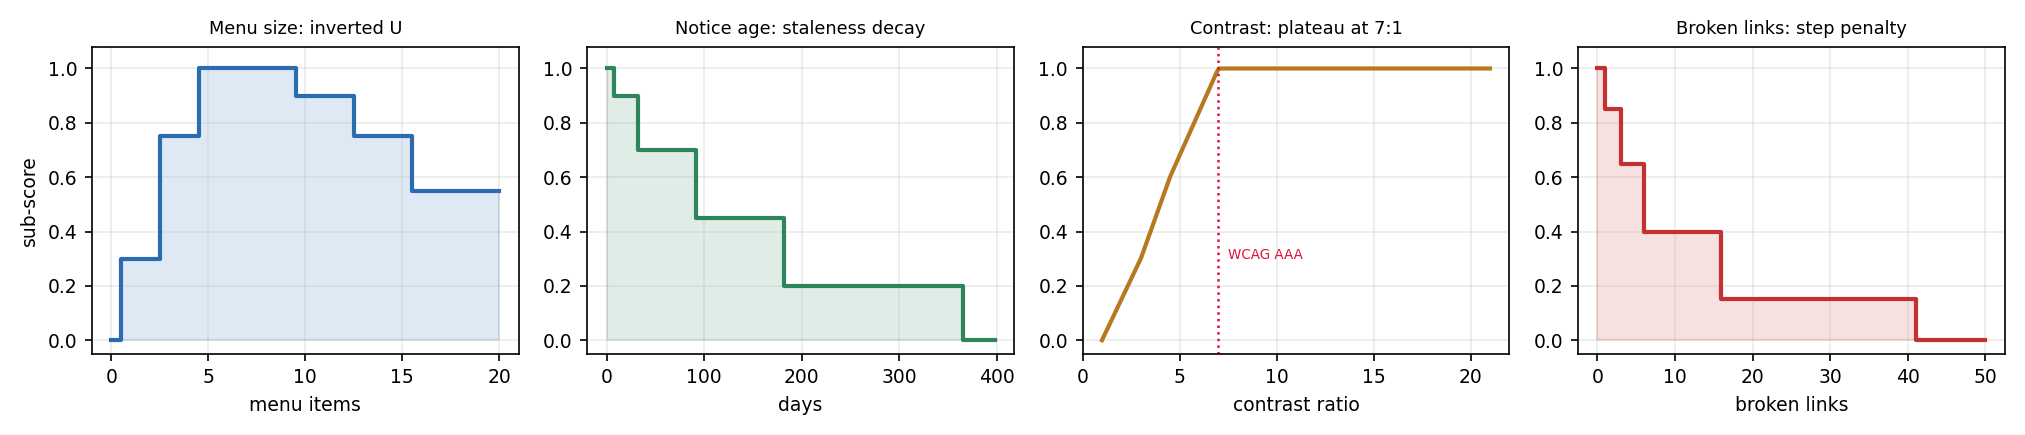
\includegraphics[width=\textwidth]{figures/fig_curves.png}
\caption{The four non-linear response curves used inside the dimension sub-scores.}
\end{figure}

\begin{itemize}
\item \textbf{Menu size --- an inverted U.} A menu with 0--2 items leads nowhere; 5--9 items
      indicates an organised site; 20 items is a wall of links. Neither ``more is better''
      nor ``less is better'' describes this, so no monotone function can represent it.
\item \textbf{Notice age --- staleness decay.} A post from last week and one from last year
      are not 51 weeks apart in value. ``Recent'' and ``abandoned'' are plateaus with a cliff
      between them.
\item \textbf{Contrast --- a plateau at 7:1.} WCAG AAA is 7:1. Beyond it, more contrast is not
      a better reading experience, so the curve stops rewarding rather than rising further.
\item \textbf{Broken links --- a step penalty.} One dead link is an oversight; forty is
      neglect. The penalty is not proportional to the count.
\end{itemize}

\subsection{The resulting target}

\begin{figure}[H]\centering
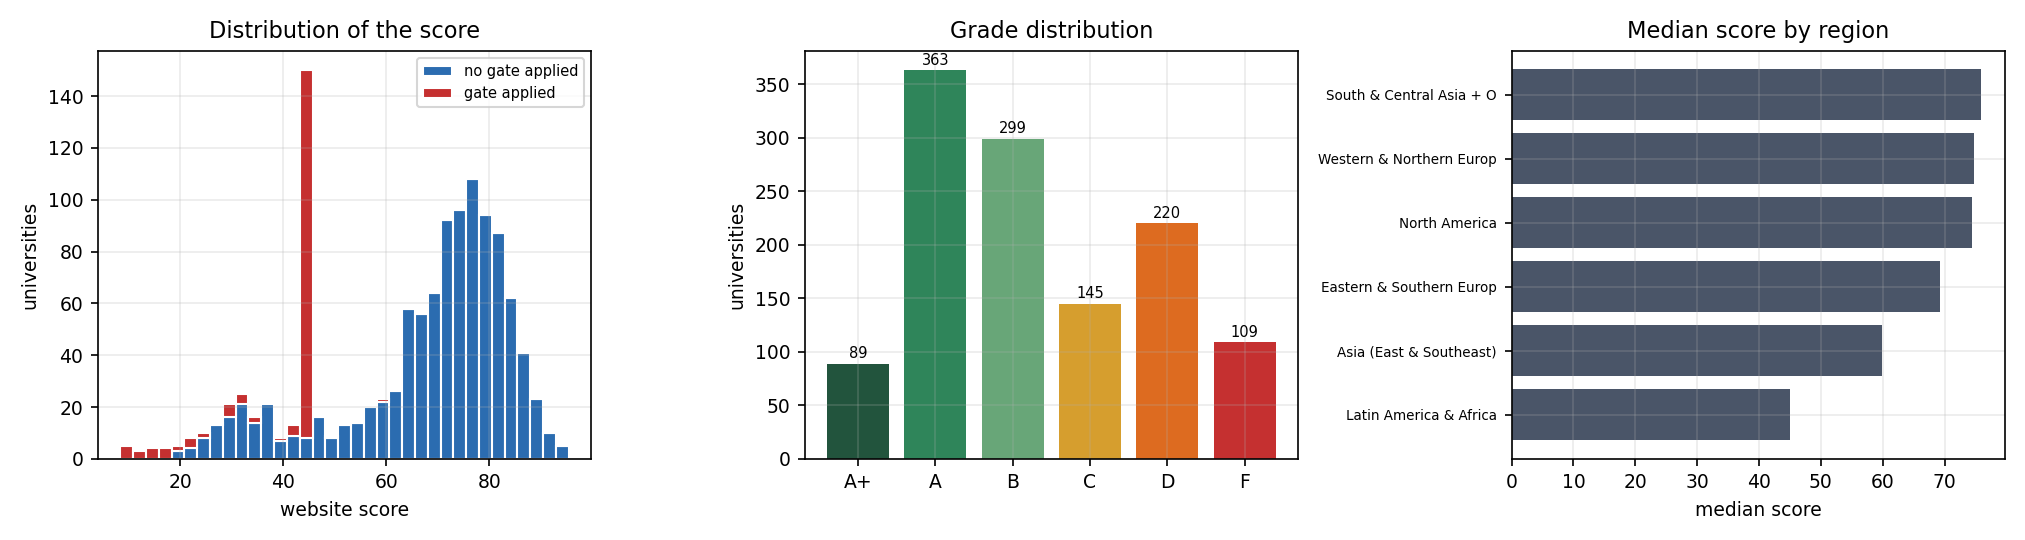
\includegraphics[width=\textwidth]{figures/fig_target.png}
\caption{The website score across 1,225 universities. The shoulder near 45 in the left panel
is the population to which a gating rule applies.}
\end{figure}

\begin{table}[H]\centering\small
\begin{tabular}{lr@{\hspace{18pt}}lr}
\toprule
Mean & 64.4 & Grade A+ ($\geq 85$) & 89 \\
Standard deviation & 18.4 & Grade A (75--85) & 363 \\
Minimum & 8.3 & Grade B (65--75) & 299 \\
Maximum & 95.4 & Grade C (50--65) & 145 \\
Universities gated & 186 & Grade D (35--50) & 220 \\
& & Grade F ($< 35$) & 109 \\
\bottomrule
\end{tabular}
\end{table}

%========================================================= 4
\section{Experimental Setup}

\subsection{Train / test split}

The dataset is split \textbf{80\% training (979 universities) / 20\% testing (246
universities)}, stratified on score band so that both halves span the full quality range, with
a fixed random seed so the split is reproducible. Stratification holds to within
1.5 percentage points in every band.

\textbf{The test set is used once}, in Section~\ref{sec:final}. No algorithm, hyper-parameter
or threshold was selected using it. Model selection and tuning use 5-fold cross-validation on
the training set only.

\subsection{Algorithms compared}

Twelve algorithms spanning six families, all trained on identical data. Feature scaling is
applied inside a pipeline for the distance-, kernel- and gradient-based methods that require
it, and deliberately not for tree methods, which are invariant to monotone rescaling.

\begin{center}\small
\begin{tabular}{ll}
\toprule
\textbf{Family} & \textbf{Algorithms} \\
\midrule
Baseline   & Mean predictor \\
Linear     & Linear Regression, Ridge ($\alpha=1$), Lasso ($\alpha=0.1$) \\
Instance   & $k$-Nearest Neighbours ($k=5$) \\
Kernel     & Support Vector Regression (RBF, $C=100$) \\
Neural     & Multi-Layer Perceptron ($128\times64$, $L_2 = 10^{-2}$) \\
Tree       & Decision Tree \\
Ensemble   & Random Forest, Extra Trees, Gradient Boosting, LightGBM \\
\bottomrule
\end{tabular}
\end{center}

\subsection{Evaluation metrics}

$R^2$ (variance explained), MAE (mean absolute error, in score points, directly
interpretable), RMSE (penalises large errors) and \textbf{Spearman $\rho$}, which measures
rank agreement and is the metric that matters most because the deliverable is a league table.

%========================================================= 5
\section{Model Comparison}
\label{sec:comparison}

\begin{table}[H]\centering\small
\caption{Twelve algorithms on the held-out test set, ordered by $R^2$. Cross-validation
figures are 5-fold on the training set only.}
\begin{tabular}{rlcccccc}
\toprule
& \textbf{Model} & \textbf{Family} & $\boldsymbol{R^2}$ & \textbf{MAE} & \textbf{RMSE} & \textbf{Spearman} & \textbf{CV }$\boldsymbol{R^2}$ \\
\midrule
1  & \textbf{LightGBM}    & ensemble & \textbf{0.992} & \textbf{1.26} & \textbf{1.71} & \textbf{0.992} & $0.986 \pm 0.001$ \\
2  & Gradient Boosting    & ensemble & 0.989 & 1.51 & 1.94 & 0.990 & $0.985 \pm 0.003$ \\
3  & Neural Net (MLP)     & neural   & 0.985 & 1.72 & 2.27 & 0.984 & $0.943 \pm 0.035$ \\
4  & Random Forest        & ensemble & 0.971 & 2.35 & 3.22 & 0.969 & $0.962 \pm 0.004$ \\
5  & SVR (RBF kernel)     & kernel   & 0.961 & 2.48 & 3.72 & 0.979 & $0.955 \pm 0.016$ \\
6  & Linear Regression    & linear   & 0.959 & 2.56 & 3.80 & 0.984 & $0.948 \pm 0.009$ \\
7  & Ridge                & linear   & 0.959 & 2.60 & 3.80 & 0.984 & $0.945 \pm 0.012$ \\
8  & Lasso                & linear   & 0.956 & 2.82 & 3.93 & 0.983 & $0.946 \pm 0.007$ \\
9  & Extra Trees          & ensemble & 0.945 & 3.13 & 4.41 & 0.939 & $0.917 \pm 0.010$ \\
10 & Decision Tree        & tree     & 0.915 & 3.78 & 5.47 & 0.926 & $0.896 \pm 0.011$ \\
11 & $k$-NN ($k=5$)       & instance & 0.786 & 5.97 & 8.67 & 0.875 & $0.770 \pm 0.025$ \\
12 & Mean baseline        & baseline & 0.000 & 15.73 & 18.76 & --- & $-0.010 \pm 0.008$ \\
\bottomrule
\end{tabular}
\end{table}

\begin{figure}[H]\centering
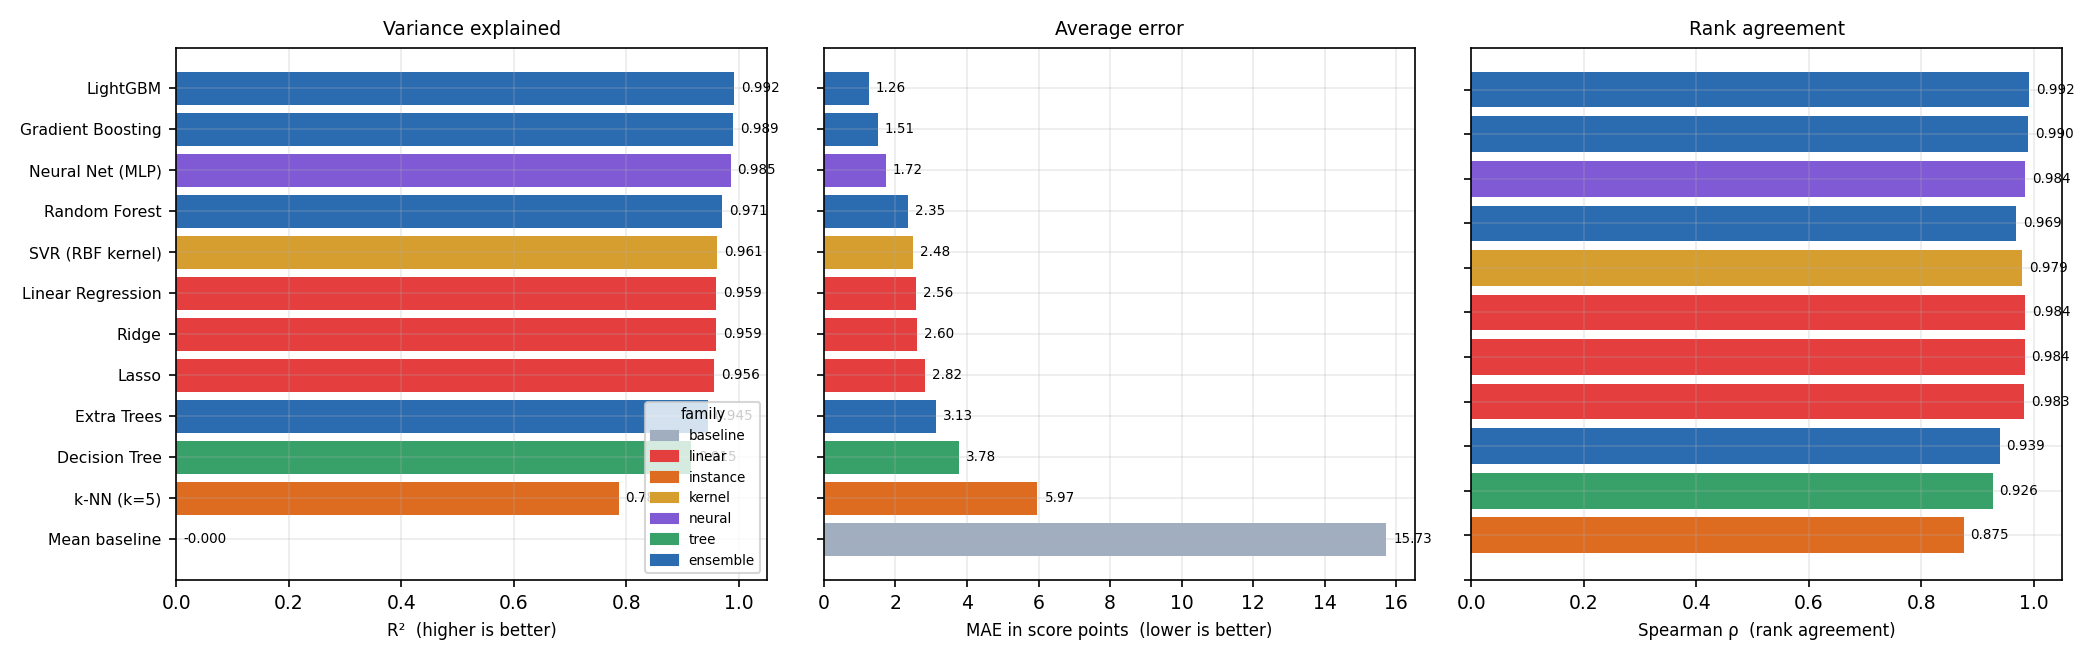
\includegraphics[width=\textwidth]{figures/fig_comparison.png}
\caption{Model comparison on the held-out test set, coloured by algorithm family.}
\end{figure}

\noindent Three observations. First, every algorithm beats the mean baseline decisively, so
the attributes carry real signal. Second, gradient-boosted ensembles lead on all four metrics.
Third, $k$-NN is the clear worst: in a 71-dimensional, largely binary space, Euclidean
distance is a poor measure of similarity --- a textbook illustration of the curse of
dimensionality.

\subsection{Cross-validation}

A single split can flatter or punish a model by chance, so the ordering was re-checked with
5-fold cross-validation on the training set alone.

\begin{figure}[H]\centering
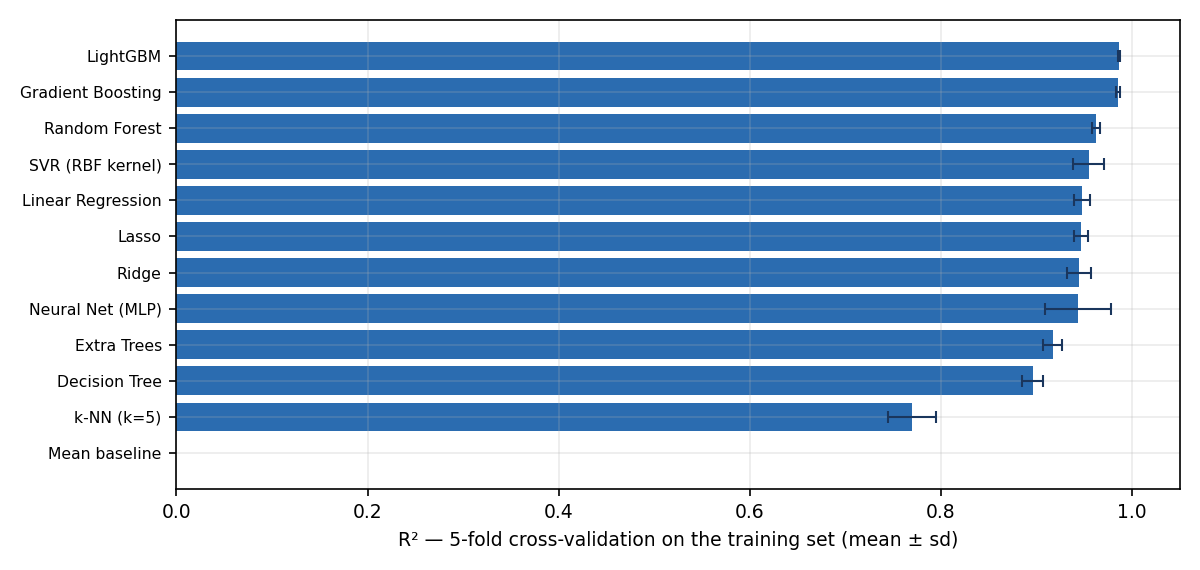
\includegraphics[width=0.78\textwidth]{figures/fig_cv.png}
\caption{Cross-validated $R^2$ (mean $\pm$ standard deviation) on the training set.}
\end{figure}

\noindent The cross-validation ordering and the test-set ordering agree at Spearman
$\rho = 0.888$, so the comparison is not an artefact of one particular split.

\begin{keybox}{A practical note on the neural network}
The MLP was the only model that required the \emph{target} to be scaled as well as the
inputs. Trained on the raw 0--100 scale, one fold in five diverged and cross-validated $R^2$
collapsed to $-0.03 \pm 1.88$. Wrapping it in a target-scaling transformer and adding $L_2$
regularisation stabilised it at $0.943 \pm 0.035$. The tree-based models needed no equivalent
care, which is part of why they are the practical choice at this dataset size.
\end{keybox}

%========================================================= 6
\section{Hyper-parameter Tuning and Final Evaluation}
\label{sec:final}

Grid search over 81 combinations, 5-fold cross-validated on the training set:

\begin{center}\small
\begin{tabular}{ll}
\toprule
\textbf{Parameter} & \textbf{Values searched (selected in bold)} \\
\midrule
\texttt{n\_estimators}      & 300, 600, \textbf{900} \\
\texttt{learning\_rate}     & 0.03, \textbf{0.05}, 0.1 \\
\texttt{num\_leaves}        & \textbf{15}, 31, 63 \\
\texttt{min\_child\_samples}& \textbf{5}, 10, 20 \\
\midrule
\multicolumn{2}{l}{Best cross-validated $R^2$: \textbf{0.9892}} \\
\bottomrule
\end{tabular}
\end{center}

\begin{table}[H]\centering
\caption{Final model on the held-out test set --- 246 universities, evaluated once.}
\begin{tabular}{lr}
\toprule
$R^2$ & \textbf{0.9931} \\
MAE (score points) & \textbf{1.11} \\
RMSE & 1.56 \\
Spearman $\rho$ & \textbf{0.9931} \\
Kendall $\tau$ & 0.9374 \\
\midrule
Predictions within $\pm 1$ point & 57.7\% \\
Predictions within $\pm 2$ points & 83.3\% \\
Predictions within $\pm 5$ points & 99.2\% \\
\bottomrule
\end{tabular}
\end{table}

\begin{figure}[H]\centering
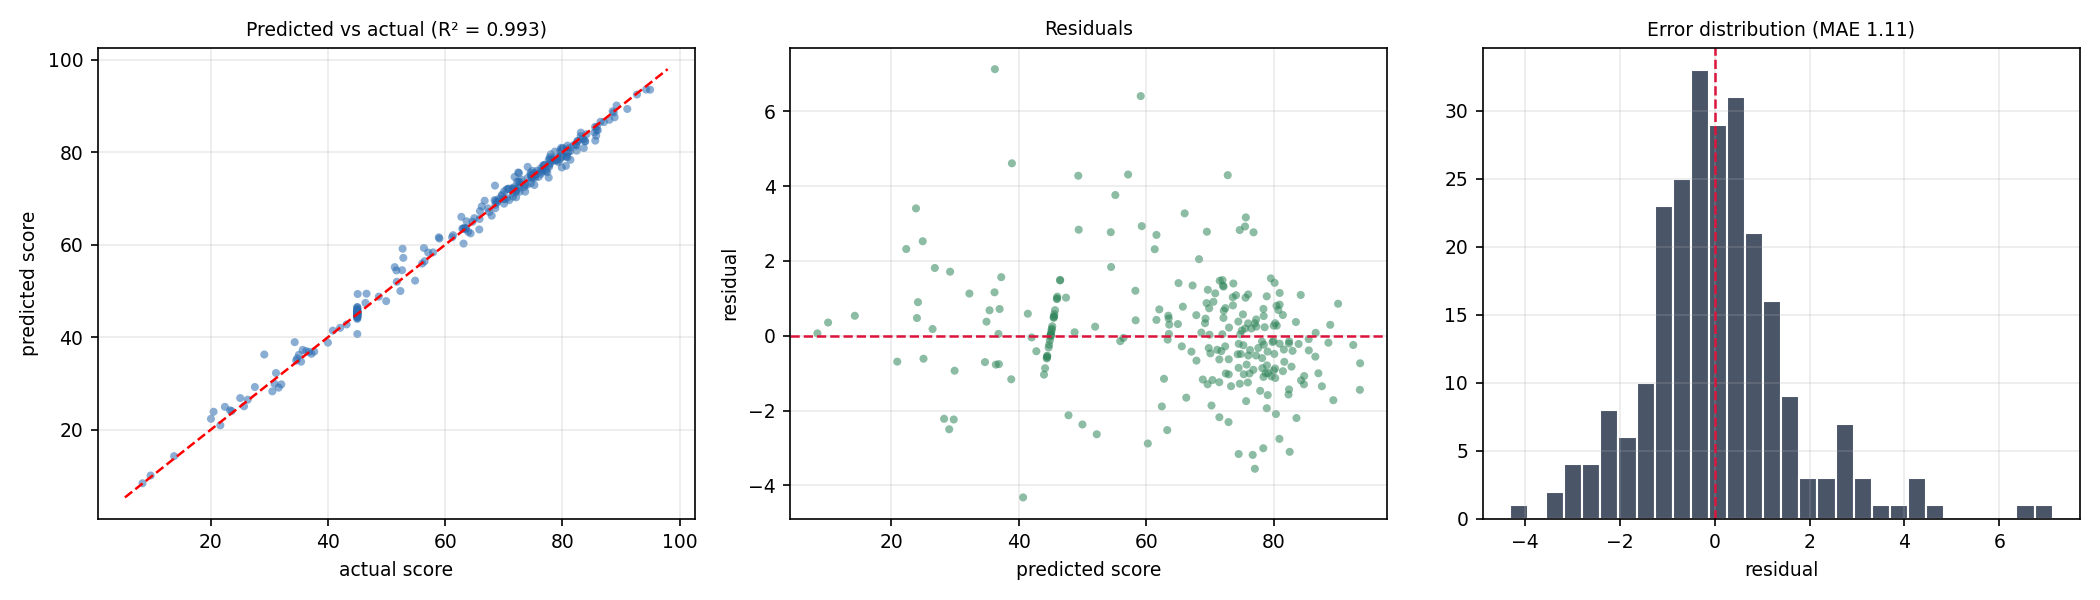
\includegraphics[width=\textwidth]{figures/fig_predictions.png}
\caption{Held-out predictions. Residuals show no systematic pattern with predicted value.}
\end{figure}

%========================================================= 7
\section{Why the Algorithms Differ}
\label{sec:why}

All twelve algorithms saw identical features and identical training data, yet $R^2$ ranged
from 0.786 to 0.992. Attributing that spread to ``model capacity'' explains nothing. The real
cause is specific, and it can be demonstrated.

The scoring model contains \textbf{gates} --- hard caps at 45 and 60 points. A linear model
computes $\sum_j \beta_j x_j$ and has no way to express \emph{``whatever else is true, stop
here''}. A decision tree does: a split is precisely that statement.

If this is the mechanism, then linear models should fail specifically on gated universities
and behave normally elsewhere. Splitting the test error accordingly:

\begin{table}[H]\centering\small
\caption{Mean absolute error on the 36 gated versus 210 ungated test universities.}
\begin{tabular}{llccc}
\toprule
\textbf{Model} & \textbf{Family} & \textbf{MAE gated} & \textbf{MAE ungated} & \textbf{ratio} \\
\midrule
Linear Regression & linear   & 6.41 & 1.91 & $3.37\times$ \\
Ridge             & linear   & 6.37 & 1.96 & $3.25\times$ \\
Lasso             & linear   & 6.47 & 2.20 & $2.94\times$ \\
SVR (RBF)         & kernel   & 4.49 & 2.14 & $2.10\times$ \\
Neural Net (MLP)  & neural   & 4.31 & 3.33 & $1.29\times$ \\
\midrule
Decision Tree     & tree     & 1.80 & 4.12 & $0.44\times$ \\
Random Forest     & ensemble & 1.05 & 2.57 & $0.41\times$ \\
Gradient Boosting & ensemble & 1.46 & 1.51 & $0.96\times$ \\
\textbf{LightGBM} & ensemble & \textbf{1.07} & \textbf{1.29} & $0.83\times$ \\
\bottomrule
\end{tabular}
\end{table}

\begin{figure}[H]\centering
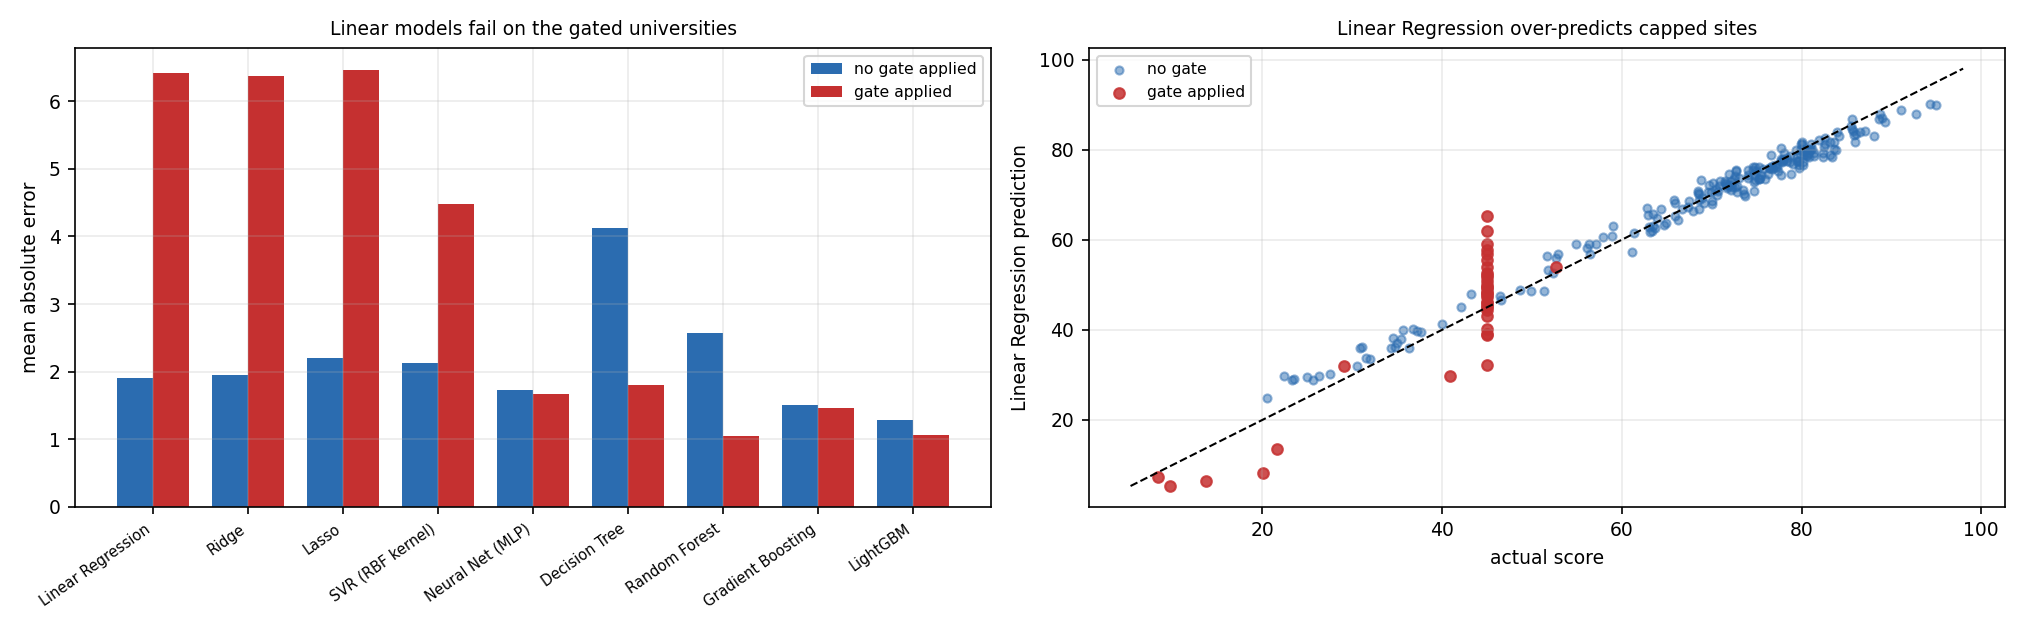
\includegraphics[width=\textwidth]{figures/fig_gates.png}
\caption{Left: error split by whether a gate applied. Right: linear regression systematically
over-predicts the capped universities (red), because it sums the content the site does have
and never applies the cap.}
\end{figure}

\begin{keybox}{The result worth taking away}
Every linear model is roughly $3\times$ worse on gated universities than on ungated ones.
Every tree-based model is \emph{as good or better} on them. The performance gap between
algorithm families in Section~\ref{sec:comparison} is therefore not a vague matter of
capacity --- it is the concrete inability of an additive model to represent a threshold, and
it is visible on 36 specific universities.
\end{keybox}

%========================================================= 8
\section{What Drives a Website's Score}
\label{sec:importance}

Feature importance is computed by \textbf{gain} --- how much each split reduced the loss ---
rather than by split count. The distinction matters: split-count importance flatters
continuous attributes, which get split many times, over binary ones, which are split once.
Under split-count importance, load time appeared to be the single most important feature; under
gain it accounts for well under 1\%.

\begin{figure}[H]\centering
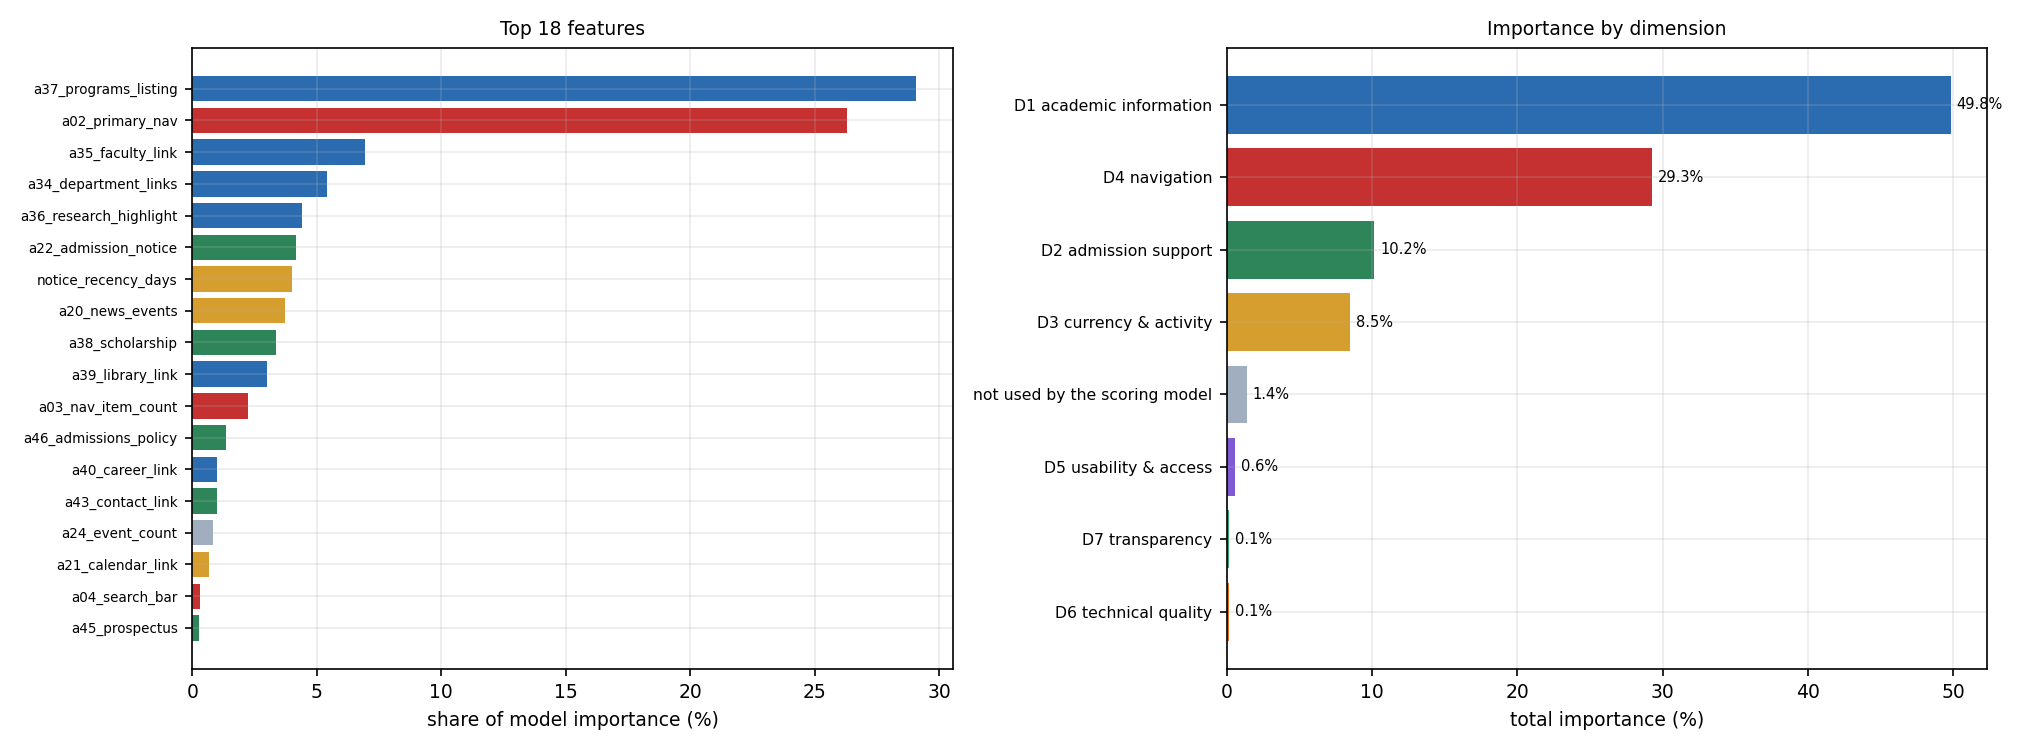
\includegraphics[width=\textwidth]{figures/fig_importance.png}
\caption{Gain-based feature importance for the tuned model, individually and aggregated by
scoring dimension.}
\end{figure}

\begin{table}[H]\centering\small
\caption{Declared dimension weight against realised model importance.}
\begin{tabular}{lrrl}
\toprule
\textbf{Dimension} & \textbf{Declared} & \textbf{Realised} & \textbf{Interpretation} \\
\midrule
$D_1$ Academic information & 28 & 49.8 & the largest single block of variation between sites \\
$D_4$ Navigation           & 15 & 29.3 & inflated because the navigation gate lives here \\
$D_2$ Admission support    & 22 & 10.2 & \\
$D_3$ Currency, activity   & 15 & 8.5  & \\
$D_5$ Usability, access    & 10 & 0.6  & near-constant across sites, so it separates almost nobody \\
$D_6$ Technical quality    & 7  & 0.1  & 98.9\% of sites use HTTPS; there is little left to explain \\
$D_7$ Transparency         & 3  & 0.1  & \\
\bottomrule
\end{tabular}
\end{table}

\noindent Two conclusions follow. First, \textbf{a declared weight is not the same as
realised influence}: a dimension can only differentiate universities to the extent that they
actually differ on it, and $D_5$--$D_7$ are close to universal. This mirrors a known result in
the website-evaluation literature, where a scheme allocating 40\% of its score to performance
was later found to drive under 3\% of its ranking variance.

Second, the model \textbf{independently recovered the gating rule}. The single attribute
\texttt{a02\_primary\_nav} accounts for \textbf{26.3\% of all gain} --- far beyond its
arithmetic contribution of 3.75 points inside $D_4$ --- because the model learned that this
one binary determines whether a 45-point ceiling applies. This is a satisfying confirmation
that the mechanism identified in Section~\ref{sec:why} is what the model actually uses.

%========================================================= 9
\section{Rankings}
\label{sec:rankings}

\begin{table}[H]\centering\small
\begin{minipage}[t]{0.53\textwidth}\centering
\textbf{Global top 10}\\[3pt]
\begin{tabular}{rlr}
\toprule
\# & University & Score \\
\midrule
1  & University of New England (AU)       & 95.4 \\
2  & University of Porto (PT)             & 95.0 \\
3  & Eotvos Lorand University (HU)        & 95.0 \\
4  & University of Strasbourg (FR)        & 94.3 \\
5  & Southern Cross University (AU)       & 93.3 \\
6  & City, University of London (UK)      & 92.9 \\
7  & Gauhati University (IN)              & 92.7 \\
8  & Nanyang Technological Univ.\ (SG)    & 92.7 \\
9  & RWTH Aachen University (DE)          & 92.6 \\
10 & Sophia University (JP)               & 92.4 \\
\bottomrule
\end{tabular}
\end{minipage}%
\begin{minipage}[t]{0.47\textwidth}\centering
\textbf{Bangladesh top 8} (of 22)\\[3pt]
\begin{tabular}{rlrr}
\toprule
\# & University & Global & Score \\
\midrule
1 & North South University & 45  & 87.4 \\
2 & RUET                   & 79  & 85.5 \\
3 & CUET                   & 114 & 83.8 \\
4 & \textbf{KUET}          & \textbf{115} & \textbf{83.8} \\
5 & AIUB                   & 136 & 83.1 \\
6 & BRAC University        & 145 & 82.7 \\
7 & Univ.\ of Professionals& 153 & 82.5 \\
8 & Patuakhali S\&T Univ.  & 235 & 80.2 \\
\bottomrule
\end{tabular}
\end{minipage}
\end{table}

\noindent Country rankings are produced for the \textbf{18 countries} with at least 20
universities in the dataset, covering 779 universities. For the 169 rows whose
\texttt{country} field holds a regional label rather than a country, no country ranking is
produced, because it would not be one.

%========================================================= 10
\section{Limitations}

These bound how the ranking should be read and are stated plainly.

\begin{enumerate}
\item \textbf{The dataset cannot see visual design.} Every attribute is a presence flag, a
      count or a measurement. Whether a page is cluttered, dated-looking or simply unpleasant
      to use is not among the 71 columns and therefore cannot be in the score. A site that
      satisfies every content requirement will score well even if a human would find it ugly.
      Closing this gap would require screenshots and human raters, not further modelling.
\item \textbf{Approximately 2\% of rows are extraction failures.} A small number of
      universities returned almost nothing to the crawler --- no navigation, no programmes, no
      contact --- which is characteristic of JavaScript-rendered pages the extractor could not
      read rather than of genuinely empty websites. These fall to the bottom of the ranking.
      The top of the ranking is unaffected, but the bottom should not be quoted without this
      caveat.
\item \textbf{The score reflects the landing page}, not the entire site and not the
      institution. An excellent admissions portal that is not linked from the front page is
      invisible to this method.
\item \textbf{The scoring weights are a documented judgement, not a measured truth.} They were
      fixed before scoring and are stated in full, but a different reasonable analyst would
      choose somewhat different weights and obtain a somewhat different ranking. The
      sensitivity of the ranking to the weights was not measured.
\item \textbf{Region and data collector are perfectly confounded.} Each of six collectors
      covered exactly one region, so regional differences in a measurement such as load time
      cannot be separated from differences in how it was measured. Load time is
      region-standardised for this reason, but the confound cannot be removed.
\item \textbf{The crawl is a single snapshot.} Websites change continuously; the freshness
      attributes in particular would differ on another day.
\end{enumerate}

%========================================================= 11
\section{Conclusion}

This project set out to automate the assessment of university website quality. We defined a
seven-dimension scoring model grounded in what a prospective student needs, applied it to
1,225 universities, and trained twelve regression algorithms to predict the resulting score
from raw landing-page attributes. The tuned LightGBM model reaches $R^2 = 0.993$ with a mean
absolute error of 1.11 points on a test set held out from every fitting and tuning decision,
and orders the universities at Spearman $\rho = 0.993$.

The comparative study is the more instructive half. Performance across the twelve algorithms
was not a smooth gradient of capability but a split along one specific structural line: models
that can represent a threshold and models that cannot. Isolating the 36 gated universities in
the test set made the mechanism visible --- linear models are $3\times$ worse on exactly those
cases and normal elsewhere --- and gain-based importance analysis confirmed that the winning
model had independently identified the gating attribute, assigning it 26\% of all loss
reduction.

Two methodological points generalise beyond this dataset. Missing values must be filled
according to what absence \emph{means}, not by a default statistic: median-filling one
attribute here would have described 468 abandoned notice boards as updated yesterday. And a
declared weight is not a realised influence: three dimensions carrying 20 points of the
scoring model account for under 1\% of what the trained model uses, simply because almost every
university scores alike on them.

\subsection*{Future work}

Adding screenshot-derived visual features and a small panel of human ratings would address the
principal limitation. Replacing the extractor with a headless browser would eliminate the
JavaScript-rendering failures. Finally, a sensitivity analysis over the dimension weights would
quantify how much of the ranking is a property of the websites and how much is a property of
our scoring choices.

%========================================================= APPENDIX
\appendix
\section{Repository contents}

\begin{table}[H]\centering\small
\begin{tabular}{ll}
\toprule
\textbf{Path} & \textbf{Contents} \\
\midrule
\texttt{data/university\_website\_scores.csv} & all 1,225 universities, scored and ranked \\
\texttt{data/train.csv}, \texttt{data/test.csv} & the 979 / 246 split (80 / 20, seed 42) \\
\texttt{data/data\_dictionary.csv} & every column, its dimension and its range \\
\texttt{data/weka/} & the same splits in ARFF format \\
\texttt{notebook/University\_Website\_Quality.ipynb} & the full analysis, executed \\
\texttt{src/build\_dataset.py} & raw file $\to$ scored dataset $\to$ splits \\
\texttt{src/make\_figures.py} & regenerates every figure in this report \\
\texttt{model/final\_model.joblib} & the tuned model \\
\texttt{results/} & model comparison, importance, metrics as CSV \\
\bottomrule
\end{tabular}
\end{table}

\noindent \textbf{Environment.} Python 3.13, pandas 2.3.3, numpy 2.4.4, scikit-learn 1.8.0,
LightGBM 4.6.0. All random seeds fixed; the pipeline is reproducible end to end by running
\texttt{src/build\_dataset.py} followed by the notebook.

\end{document}
